\documentclass[11pt,paper=a4,answers]{exam}
\usepackage{graphicx,lastpage}
\usepackage{upgreek}
\usepackage{censor}
\usepackage{gensymb}
\usepackage{amsmath}
\usepackage{multicol}
\usepackage{enumitem}
 \usepackage{pgfplots}
\pgfplotsset{compat=1.18}
\usepackage{tasks}
\usepackage{adjustbox}
\usepackage{xcolor}
\usepackage{tfrupee}
\setlength{\voffset}{0.25in}
\usepackage{tabularx}
\newcolumntype{Y}{>{\centering\arraybackslash}X}
%==============================================================
% Customise Non-Essential Packages Below
% =============================================================
\usepackage[most]{tcolorbox}
\usepackage{eso-pic}
\usepackage{tikz}
\AddToShipoutPictureBG{%
\begin{tikzpicture}[remember picture,overlay]
\foreach \x in {-8,-4,0,4,8,12,16,20}
\foreach \y in {-8,-4,0,4,8,12,16,20} {
\node[opacity=0.05,rotate=45,anchor=center] at ([xshift=\x cm,yshift=\y cm]current page.center) {%
\begin{minipage}{2cm}
\centering
\includegraphics[width=2cm]{images/logo_black.png}\\
\small preppeo.com
\end{minipage}%
};
}
\end{tikzpicture}%
}
\printanswers

%==============================================================
% Customise Non-Essential Packages Above
% =============================================================
\definecolor{svgray}{rgb}{0.90, 0.90, 0.90}
\graphicspath{{images/}}

\usepackage[normalem]{ulem}
\renewcommand\ULthickness{1pt}   %%---> For changing thickness of underline
\setlength\ULdepth{3.5ex}%\maxdimen ---> For changing depth of underline
\renewcommand{\baselinestretch}{1}
\chead{
\includegraphics[scale=0.1,height=2cm ]{logo.png}
}
\pagestyle{empty}

\pagestyle{headandfoot}
\headrule
\cfoot{W: https://preppeo.com; M: +91-8130711689}

\begin{document}
%==============================================================
% Customise Question paper details below this
% =============================================================
\begin{center}
    \centering
    \renewcommand{\arraystretch}{1.5}
    \begin{tabularx}{\textwidth}{YYY}
    & \normalsize\bf{{\Large{{Quantitative Reasoning}}}} & \\
    By Preppeo & \normalsize\bf{MOCK } & GRE\\
    \normalsize{\textbf{Questions:} 15 (Section 2 : 15} & \normalsize{\textbf{Marks:} 15 } & \normalsize{\textbf{Time:}  minutes } \\
    \end{tabularx}
\end{center}
\par\noindent\rule{\textwidth}{1pt}
% =============================================================
% Customise Question paper details above this
% =============================================================

\begin{questions}
\pointsinrightmargin
\pointsdroppedatright
\marksnotpoints
\pointpoints{mark}{marks}
\pointformat{\boldmath\themarginpoints}
\bracketedpoints

% =============================================================
% Question Begin
% =============================================================

\section*{Section 2 - Mock 6 Set 3 (Medium-Hard)}

% --- QUANTITY COMPARISON (5 QUESTIONS) ---

%Q: 1
\question
\[ 15! \text{ is divisible by } 3^x 5^y \]
where $x$ and $y$ are positive integers.
\vspace{5pt}\\
\textbf{Quantity A: } The greatest possible value for $x$ \\
\vspace{5pt}
\textbf{Quantity B: } Twice the greatest possible value for $y$

\begin{tasks}(1)
\task[A)] Quantity A is greater
\task[B)] Quantity B is greater
\task[C)] The two quantities are equal
\task[D)] The relationship cannot be determined
\end{tasks}

\begin{solution}
To find the greatest power of a prime $p$ that divides $n!$, use Legendre's Formula.
\vspace{5pt}
\begin{center}
Find $x$ for prime 3: $\lfloor 15/3 \rfloor + \lfloor 15/9 \rfloor = 5 + 1 = 6$
\vspace{5pt}
Find $y$ for prime 5: $\lfloor 15/5 \rfloor = 3$
\end{center}
\vspace{5pt}
Quantity A is 6. 
\vspace{5pt}
Quantity B is $2 \times 3 = 6$.
\vspace{5pt}
Comparing 6 and 6, the quantities are equal.

Answer: \colorbox{yellow!100}{C}
\end{solution}

\vspace{1cm}

%Q: 2
\question
\begin{center}
\begin{tikzpicture}[scale=0.8]
    \draw[thick] (0,0) coordinate (A) -- (5,0) coordinate (C) -- (2,4) coordinate (B) -- cycle;
    \draw[thick, blue] (1,2) coordinate (D) -- (4,2) coordinate (E);
    \node[left] at (A) {$A$};
    \node[right] at (C) {$C$};
    \node[above] at (B) {$B$};
    \node[left, blue] at (D) {$D$};
    \node[right, blue] at (E) {$E$};
\end{tikzpicture}
\end{center}
In the triangle $ABC$, $DE \parallel AC$. The area of triangle $BDE$ is 16 and the ratio $BD/BA = 2/3$.
\vspace{5pt}\\
\textbf{Quantity A: } The area of triangle $ABC$ \\
\vspace{5pt}
\textbf{Quantity B: } 36

\begin{tasks}(1)
\task[A)] Quantity A is greater
\task[B)] Quantity B is greater
\task[C)] The two quantities are equal
\task[D)] The relationship cannot be determined
\end{tasks}

\begin{solution}
Since $DE \parallel AC$, triangles $BDE$ and $BAC$ are similar by AA similarity.
\vspace{5pt}
\begin{center}
The ratio of the areas of two similar triangles is the square of the ratio of their corresponding sides.
\vspace{5pt}
$\dfrac{\text{Area}(BDE)}{\text{Area}(BAC)} = \left( \dfrac{BD}{BA} \right)^2$
\vspace{5pt}
$\dfrac{16}{\text{Area}(ABC)} = \left( \dfrac{2}{3} \right)^2 = \dfrac{4}{9}$
\vspace{5pt}
$4 \times \text{Area}(ABC) = 16 \times 9 = 144$
\vspace{5pt}
$\text{Area}(ABC) = 144 / 4 = 36$
\end{center}
\vspace{5pt}
Quantity A is 36 and Quantity B is 36.

Answer: \colorbox{yellow!100}{C}
\end{solution}

\vspace{1cm}

%Q: 3
\question
The median of a set of 7 distinct integers is 20. 
\vspace{5pt}\\
\textbf{Quantity A: } The average (arithmetic mean) of the integers \\
\vspace{5pt}
\textbf{Quantity B: } 20

\begin{tasks}(1)
\task[A)] Quantity A is greater
\task[B)] Quantity B is greater
\task[C)] The two quantities are equal
\task[D)] The relationship cannot be determined
\end{tasks}

\begin{solution}
Let the set be $\{x_1, x_2, x_3, 20, x_5, x_6, x_7\}$.
\vspace{5pt}
\begin{center}
Case 1: The numbers above 20 are very large (e.g., 200, 300, 400). The average will be much greater than 20.
\vspace{5pt}
Case 2: The numbers below 20 are very small (e.g., -100, -200, -300). The average will be much less than 20.
\end{center}
\vspace{5pt}
Because the mean can be influenced by outliers while the median remains fixed, the relationship cannot be determined.

Answer: \colorbox{yellow!100}{D}
\end{solution}

\vspace{1cm}

%Q: 4
\question
$k$ is a positive integer.
\vspace{5pt}\\
\textbf{Quantity A: } The units digit of $7^{4k+2}$ \\
\vspace{5pt}
\textbf{Quantity B: } The units digit of $3^{4k+2}$

\begin{tasks}(1)
\task[A)] Quantity A is greater
\task[B)] Quantity B is greater
\task[C)] The two quantities are equal
\task[D)] The relationship cannot be determined
\end{tasks}

\begin{solution}
Analyze the units digit cycles for both bases.
\vspace{5pt}
\begin{center}
Cycle for 7: $7^1=7, 7^2=9, 7^3=3, 7^4=1$ (Length 4).
\vspace{5pt}
Since the exponent $4k+2$ divided by 4 leaves a remainder of 2, the units digit is 9.
\vspace{10pt}
Cycle for 3: $3^1=3, 3^2=9, 3^3=7, 3^4=1$ (Length 4).
\vspace{5pt}
Since the exponent $4k+2$ divided by 4 leaves a remainder of 2, the units digit is 9.
\end{center}
\vspace{5pt}
Both quantities are equal to 9.

Answer: \colorbox{yellow!100}{C}
\end{solution}

\vspace{1cm}

%Q: 5
\question
The price of a stock rose by 25 percent and then decreased by $y$ percent After the decrease, the stock was back to its original price.
\vspace{5pt}
\textbf{Quantity A: } $y$ \\
\vspace{5pt}
\textbf{Quantity B: } 25

\begin{tasks}(1)
\task[A)] Quantity A is greater
\task[B)] Quantity B is greater
\task[C)] The two quantities are equal
\task[D)] The relationship cannot be determined
\end{tasks}

\begin{solution}
Let the original price be 100.
\vspace{5pt}
\begin{center}
After 25\% increase: $100 \times 1.25 = 125$
\vspace{5pt}
To return to 100, the price must decrease by 25.
\vspace{5pt}
$y = (25 / 125) \times 100 = (1/5) \times 100 = 20$
\end{center}
\vspace{5pt}
Quantity A is 20 and Quantity B is 25. Quantity B is greater.

Answer: \colorbox{yellow!100}{B}
\end{solution}

\vspace{1cm}

% --- MCQ SINGLE CHOICE (5 QUESTIONS) ---

%Q: 6
\question
A chemist currently has 30 ounces of a solution, 10 of which are acetone. How many ounces of pure acetone must she add to the current mixture to attain a 50/50 mixture of acetone and water?

\begin{tasks}(1)
\task[A)] 5 \task[B)] 10 \task[C)] 15 \task[D)] 20 \task[E)] 25
\end{tasks}

\begin{solution}
\begin{center}
Current water $= 30 - 10 = 20 \text{ ounces}$
\vspace{5pt}
In a 50/50 mixture, the amount of acetone must equal the amount of water.
\vspace{5pt}
Target acetone $= 20 \text{ ounces}$
\vspace{5pt}
Amount to add $= 20 - 10 = 10 \text{ ounces}$
\end{center}

Answer: \colorbox{yellow!100}{B}
\end{solution}

\vspace{1cm}

%Q: 7
\question
In a parking lot, 1/3 of the vehicles are black and 1/5 of the remainder are white. If there are 30 white vehicles, how many total vehicles could be parked on the lot? (Wait, adjusted for consistency with Mock logic). 
If 1/3 are black and 1/5 are white, what is the minimum number of vehicles in the lot?

\begin{tasks}(1)
\task[A)] 8 \task[B)] 12 \task[C)] 15 \task[D)] 30 \task[E)] 45
\end{tasks}

\begin{solution}
The total number of vehicles must be divisible by the denominators of the fractions used to describe the parts.
\vspace{5pt}
\begin{center}
Denominators are 3 and 5.
\vspace{5pt}
The least common multiple is 15.
\end{center}
\vspace{5pt}
At a minimum, there must be 15 vehicles to satisfy the fractional counts as whole numbers.

Answer: \colorbox{yellow!100}{C}
\end{solution}

\vspace{1cm}

%Q: 8
\question
\begin{center}
\begin{tikzpicture}
    \draw[thick] (0,0) -- (6,0) node[midway, below] {$BC=12$} -- (6,4) -- cycle;
    \draw (5.7,0) -- (5.7,0.3) -- (6,0.3);
    \node[left] at (0,0) {$B$};
    \node[right] at (6,4) {$l$};
\end{tikzpicture}
\end{center}
In the coordinate system above, the slope of line $l$ is $2/3$. If the length of $BC$ is 12, what is the length of $AB$?

\begin{tasks}(1)
\task[A)] 4 \task[B)] 6 \task[C)] 8 \task[D)] 12 \task[E)] 18
\end{tasks}

\begin{solution}
\begin{center}
$\text{Slope} = \text{Rise} / \text{Run} = AB / BC$
\vspace{5pt}
$2/3 = AB / 12$
\vspace{5pt}
$3 \times AB = 24 \implies AB = 8$
\end{center}

Answer: \colorbox{yellow!100}{C}
\end{solution}

\vspace{1cm}

%Q: 9
\question
If $f(x) = x^2 - 4x$, what is the value of $f(x+2) - f(x-2)$?

\begin{tasks}(1)
\task[A)] $8x$ \task[B)] $8x-16$ \task[C)] $4x-8$ \task[D)] $16x$ \task[E)] $0$
\end{tasks}

\begin{solution}
\begin{center}
$f(x+2) = (x+2)^2 - 4(x+2) = x^2 + 4x + 4 - 4x - 8 = x^2 - 4$
\vspace{5pt}
$f(x-2) = (x-2)^2 - 4(x-2) = x^2 - 4x + 4 - 4x + 8 = x^2 - 8x + 12$
\vspace{5pt}
Subtracting: $(x^2 - 4) - (x^2 - 8x + 12) = 8x - 16$
\end{center}

Answer: \colorbox{yellow!100}{B}
\end{solution}

\vspace{1cm}

%Q: 10
\question
A square is inscribed in a circle with an area of $64\pi$. What is the area of the square?

\begin{tasks}(1)
\task[A)] 64 \task[B)] 96 \task[C)] 128 \task[D)] 160 \task[E)] 256
\end{tasks}

\begin{solution}
\begin{center}
$\pi r^2 = 64\pi \implies r^2 = 64 \implies r = 8$
\vspace{5pt}
The diameter of the circle is $2 \times 8 = 16$.
\vspace{5pt}
The diameter of the circle is the diagonal ($d$) of the inscribed square.
\vspace{5pt}
Area of square $= d^2 / 2 = 16^2 / 2 = 256 / 2 = 128$
\end{center}

Answer: \colorbox{yellow!100}{C}
\end{solution}

\vspace{1cm}

% --- MCQ MULTIPLE CHOICE (1 QUESTION) ---

%Q: 11
\question
If $xz=12$ and $yz=24$, and $z \neq 0$, which of the following could be the value of $x-y$?
Indicate \textbf{all} such values.

\begin{tasks}(1)
\task[A)] -12
\task[B)] 12
\task[C)] -6
\task[D)] 6
\end{tasks}

\begin{solution}
\begin{center}
$x = 12/z$ and $y = 24/z$
\vspace{5pt}
$x - y = 12/z - 24/z = -12/z$
\vspace{5pt}
If $z=1$, $x-y = -12$.
\vspace{5pt}
If $z=-1$, $x-y = 12$.
\vspace{5pt}
If $z=2$, $x-y = -6$.
\vspace{5pt}
If $z=-2$, $x-y = 6$.
\end{center}
All four values are possible depending on the integer $z$.

Answer: \colorbox{yellow!100}{A, B, C, D}
\end{solution}

\vspace{1cm}

% --- INPUT QUESTION (1 QUESTION) ---

%Q: 12
\question
What is the units digit of $7^{100}$?

\begin{solution}
\begin{center}
Cycle for 7: $7, 9, 3, 1$. (Length 4).
\vspace{5pt}
$100 \div 4 = 25$ with remainder 0.
\vspace{5pt}
The 4th digit in the cycle is 1.
\end{center}

Answer: \colorbox{yellow!100}{1}
\end{solution}

\vspace{1cm}

% --- DATA INTERPRETATION (3 QUESTIONS) ---
\textbf{Questions 13-15 refer to the following graph.}

\begin{center}
\begin{tikzpicture}
\begin{axis}[
    title={Departmental Performance},
    xlabel={Department},
    ylabel={Units/Member},
    symbolic x coords={A, B, C, D},
    xtick=data,
    ymin=0, ymax=20,
    grid=major,
    width=8cm, height=6cm
]
\addplot[ybar, fill=blue!30] coordinates {(A,12) (B,15) (C,18) (D,10)};
\end{axis}
\end{tikzpicture}
\end{center}

%Q: 13
\question
If Department C has 5 members, what is the total number of units produced by Department C?

\begin{tasks}(1)
\task[A)] 18 \task[B)] 36 \task[C)] 72 \task[D)] 90 \task[E)] 108
\end{tasks}

\begin{solution}
\begin{center}
Units per member in Dept C $= 18$
\vspace{5pt}
Total units $= 18 \times 5 = 90$
\end{center}

Answer: \colorbox{yellow!100}{D}
\end{solution}

\vspace{1cm}

%Q: 14
\question
The performance of Department B is what percent greater than that of Department D?

\begin{tasks}(1)
\task[A)] 5% \task[B)] 15% \task[C)] 25% \task[D)] 50% \task[E)] 75%
\end{tasks}

\begin{solution}
\begin{center}
Dept B $= 15$, Dept D $= 10$.
\vspace{5pt}
Increase $= 15 - 10 = 5$.
\vspace{5pt}
Percent Greater $= (5 / 10) \times 100 = 50\%$
\end{center}

Answer: \colorbox{yellow!100}{D}
\end{solution}

\vspace{1cm}

%Q: 15
\question
Which of the following statements about the departments are true?
Indicate \textbf{all} such statements.

\begin{tasks}(1)
\task[A)] The average performance of the four departments is 13.75.
\task[B)] Department C is the most productive per member.
\task[C)] Department A produced more total units than Department D.
\end{tasks}

\begin{solution}
\begin{center}
A: Average $= (12+15+18+10) / 4 = 55 / 4 = 13.75$. (True)
\vspace{5pt}
B: Dept C has the highest bar at 18. (True)
\vspace{5pt}
C: We do not know the number of members in Dept A or D, so total units cannot be compared. (False)
\end{center}

Answer: \colorbox{yellow!100}{A, B}
\end{solution}

% =============================================================
% Question End
% =============================================================

\end{questions}
\begin{center}
\rule{.5\textwidth}{1pt}
\end{center}
\end{document}
